\subsection{Método de Newton-Raphson}

El método de Newton-Raphson es un algoritmo iterativo para encontrar raíces de funciones reales. Utiliza la derivada de la función para aproximar la raíz a partir de un valor inicial \cite{newtons-method}. Según \cite{newton-optimization} el método de Newton es una de las herramientas fundamentales en análisis numérico, investigación de operaciones, optimización y control. Tiene numerosas aplicaciones en la ciencia de la administración, la investigación industrial y financiera, y la minería de datos.

\subsubsection{Fundamento teórico}

El método se basa en la aproximación lineal de la función mediante su serie de Taylor. Si $x_n$ es una aproximación a la raíz, entonces la siguiente aproximación $x_{n+1}$ se obtiene encontrando donde la línea tangente a la curva en el punto $(x_n, f(x_n))$ cruza el eje $x$.

\begin{figure}[h]
	\centering
	\shorthandoff{<>}
	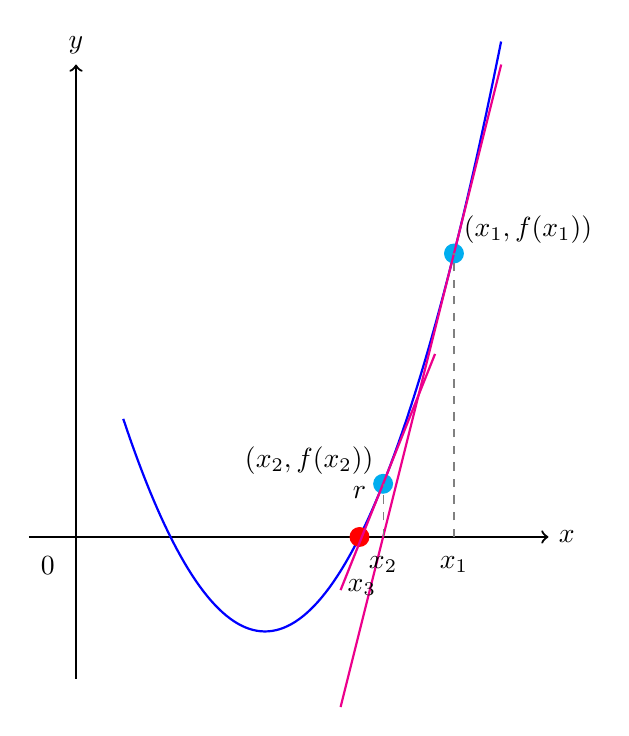
\begin{tikzpicture}[scale=1.2]
		% Axes
		\draw[->, thick] (-0.5,0) -- (5,0) node[right] {$x$};
		\draw[->, thick] (0,-1.5) -- (0,5) node[above] {$y$};
		\node at (-0.3,-0.3) {$0$};

		% Plot the function f(x) = (x-2)^2 - 1
		\draw[blue, thick, domain=0.5:4.5, samples=100] plot (\x, {(\x-2)^2 - 1});

		% Newton-Raphson iterations
		% For f(x) = (x-2)^2 - 1, f'(x) = 2(x-2)

		% Starting point x1
		\def\xone{4}
		\pgfmathsetmacro{\yone}{(\xone-2)^2 - 1}  % f(4) = 3
		\pgfmathsetmacro{\slopeone}{2*(\xone-2)}  % f'(4) = 4
		\pgfmathsetmacro{\xtwo}{\xone - \yone/\slopeone}  % x2 = 4 - 3/4 = 3.25

		% Second point x2
		\pgfmathsetmacro{\ytwo}{(\xtwo-2)^2 - 1}  % f(3.25)
		\pgfmathsetmacro{\slopetwo}{2*(\xtwo-2)}  % f'(3.25)
		\pgfmathsetmacro{\xthree}{\xtwo - \ytwo/\slopetwo}  % x3

		% Third iteration
		\pgfmathsetmacro{\ythree}{(\xthree-2)^2 - 1}
		\pgfmathsetmacro{\slopethree}{2*(\xthree-2)}
		\pgfmathsetmacro{\xfour}{\xthree - \ythree/\slopethree}  % x4

		% Root r (approximately at x=3, the right root)
		\def\xroot{3}
		\pgfmathsetmacro{\yroot}{(\xroot-2)*(\xroot-2) - 1}

		% Plot points on curve
		\fill[cyan] (\xone,\yone) circle (3pt);
		\fill[cyan] (\xtwo,\ytwo) circle (3pt);
		\fill[red] (\xroot,\yroot) circle (3pt);

		% Tangent lines (magenta) - properly calculated
		% Tangent at x1: y - f(x1) = f'(x1)(x - x1)
		% Rearranged: y = f'(x1)*x + (f(x1) - f'(x1)*x1)
		\draw[magenta, thick, domain=2.8:4.5] plot (\x, {\slopeone*(\x - \xone) + \yone});

		% Tangent at x2
		\draw[magenta, thick, domain=2.8:3.8] plot (\x, {\slopetwo*(\x - \xtwo) + \ytwo});

		% Vertical dashed lines
		\draw[gray, dashed] (\xone,0) -- (\xone,\yone);
		\draw[gray, dashed] (\xtwo,0) -- (\xtwo,\ytwo);

		% Labels for points
		\node[above right] at (\xone,\yone) {$(x_1, f(x_1))$};
		\node[above left] at (\xtwo,\ytwo) {$(x_2, f(x_2))$};
		\node[above] at (\xroot,0.3) {$r$};

		% Labels on x-axis (with adjusted positions to avoid overlap)
		\node[below] at (\xthree,-0.35) {$x_3$};
		\node[below] at (\xtwo,-0.1) {$x_2$};
		\node[below] at (\xone,-0.1) {$x_1$};

	\end{tikzpicture}
	\shorthandon{<>}
	\caption{Visualización del método de Newton-Raphson}
\end{figure}

\subsubsection{Fórmula iterativa}

La fórmula de Newton-Raphson es:
\begin{equation}
	x_{n+1} = x_n - \frac{f(x_n)}{f'(x_n)}
\end{equation}

Geométricamente, esto representa extender la tangente a la curva en el punto $(x_n, f(x_n))$ hasta que intersecte el eje $x$.

\subsubsection{Algoritmo}

\begin{enumerate}
	\item Elegir un valor inicial $x_0$ cercano a la raíz esperada
	\item Calcular $f(x_n)$ y $f'(x_n)$
	\item Verificar que $f'(x_n) \neq 0$
	\item Calcular la siguiente aproximación: $x_{n+1} = x_n - \frac{f(x_n)}{f'(x_n)}$
	\item Verificar el criterio de convergencia: $|x_{n+1} - x_n| < \epsilon$ o $|f(x_{n+1})| < \epsilon$
	\item Si no se cumple el criterio, repetir desde el paso 2
\end{enumerate}

\subsubsection{Ventajas y desventajas}

\textbf{Ventajas:}
\begin{itemize}
	\item Convergencia cuadrática cuando se está cerca de la raíz
	\item Requiere menos iteraciones que bisección
	\item Muy preciso cuando converge
\end{itemize}

\textbf{Desventajas:}
\begin{itemize}
	\item Requiere calcular la derivada $f'(x)$
	\item No garantiza convergencia si la elección inicial es mala
	\item Puede diverger o ciclar si $f'(x)$ es muy pequeña
	\item Sensible a la elección del punto inicial
\end{itemize}

\subsubsection{Condiciones de convergencia}

El método converge si:
\begin{itemize}
	\item La función es continuamente diferenciable
	\item La derivada no se anula en la vecindad de la raíz
	\item El valor inicial $x_0$ está suficientemente cerca de la raíz
\end{itemize}
